\section{Token Distribution Architecture}


\subsection{Fixed Supply Model}

Zoo implements a \textbf{non-inflationary} token model with absolute cap:

\begin{equation}
S_{\text{total}} = 2 \times 10^{12} \text{ } \KEEPER \text{ tokens (fixed permanently)}
\end{equation}

No mechanism exists for minting additional tokens. This contrasts with inflationary models (Ethereum pre-merge, Solana) and ensures long-term scarcity.

\subsection{Allocation Breakdown}

The 2T supply divides into two equal tranches:

\begin{equation}
S_{\text{total}} = S_{\DAO} + S_{\text{community}}
\end{equation}

where:
\begin{align}
S_{\DAO} &= 1 \times 10^{12} \text{ (DAO Treasury)} \\
S_{\text{community}} &= 1 \times 10^{12} \text{ (Community Airdrop)}
\end{align}

\subsubsection{DAO Treasury (1T Tokens)}

The DAO treasury serves five functions:

\begin{enumerate}
\item \textbf{Ecosystem Grants}: Funding developers, researchers, and community builders (30\% allocation target)
\item \textbf{Liquidity Provision}: Ensuring $\KEEPER$ can be exchanged for stablecoins/other assets (20\% allocation)
\item \textbf{Validator Subsidies}: Bootstrapping network security until fee revenue suffices (15\% allocation)
\item \textbf{Strategic Reserves}: Long-term operational sustainability (25\% allocation)
\item \textbf{Emergency Fund}: Black swan events, critical upgrades (10\% allocation)
\end{enumerate}

Treasury management follows strict DAO governance (Section 9), requiring 66\% supermajority for expenditures exceeding 0.1\% (1B tokens) of reserves.

\subsubsection{Community Airdrop (1T Tokens)}

The community airdrop distributed tokens based on four criteria:

\begin{equation}
A_i = w_1 \cdot E_i + w_2 \cdot D_i + w_3 \cdot C_i + w_4 \cdot R_i
\end{equation}

where:
\begin{itemize}
\item $A_i$: Airdrop allocation for participant $i$
\item $E_i$: Early engagement score (account age, activity)
\item $D_i$: Data contribution score (datasets, annotations, feedback)
\item $C_i$: Code contribution score (GitHub commits, PRs, documentation)
\item $R_i$: Referral score (community growth facilitation)
\item $w_1, w_2, w_3, w_4$: Weighting factors (sum to 1)
\end{itemize}

Actual weights applied:
\begin{align}
w_1 &= 0.30 \text{ (early engagement)} \\
w_2 &= 0.40 \text{ (data contribution)} \\
w_3 &= 0.20 \text{ (code contribution)} \\
w_4 &= 0.10 \text{ (referrals)}
\end{align}

This formula incentivizes genuine participation over Sybil attacks. Data contribution weighted highest reflects Zoo's core value proposition: training-free GRPO requires quality semantic experiences.

\subsection{Airdrop Distribution Statistics}

The September 2025 airdrop achieved remarkable decentralization:

\begin{table}[h]
\centering
\begin{tabular}{lc}
\toprule
\textbf{Metric} & \textbf{Value} \\
\midrule
Total Recipients & 87,341 \\
Countries Represented & 142 \\
Median Allocation & 8,726,000 $\KEEPER$ \\
Mean Allocation & 11,449,000 $\KEEPER$ \\
Largest Single Allocation & 2,150,000,000 $\KEEPER$ (0.215\%) \\
Top 1\% Holdings & 14.2\% \\
Top 10\% Holdings & 38.7\% \\
Gini Coefficient & 0.61 \\
\bottomrule
\end{tabular}
\caption{Zoo Network airdrop distribution statistics (September 2025)}
\label{tab:airdrop_stats}
\end{table}

For comparison, typical cryptocurrency Gini coefficients:
\begin{itemize}
\item Bitcoin: 0.88 (highly concentrated)
\item Ethereum: 0.79 (concentrated)
\item Solana: 0.85 (very concentrated)
\item Zoo: 0.61 (\textbf{significantly more equitable})
\end{itemize}

The lower Gini coefficient demonstrates that Zoo achieved superior decentralization despite zero mining period or ICO stages that typically drive early concentration.

\subsection{No Private Sales, No VCs}

Zoo's 100\% airdrop eliminates structural advantages that plague blockchain projects:

\begin{table}[h]
\centering
\small
\begin{tabular}{lcccc}
\toprule
\textbf{Project} & \textbf{Private Sale?} & \textbf{VC Allocation} & \textbf{Public Access} & \textbf{Lockup Period} \\
\midrule
RENDER & Yes (\$0.025/token) & 30\% & ICO (\$0.25/token) & 2 years \\
Bittensor & Mining only & 0\% & Fair mine & Variable \\
Fetch.ai & Yes (\$0.01/token) & 40\% & ICO (\$0.10/token) & 1-3 years \\
NEAR & Yes (\$0.04/token) & 35\% & ICO (\$0.40/token) & 1-4 years \\
\textbf{Zoo} & \textbf{No} & \textbf{0\%} & \textbf{100\% airdrop} & \textbf{None} \\
\bottomrule
\end{tabular}
\caption{Private sale comparison across AI blockchain projects}
\label{tab:private_sales}
\end{table}

In traditional models, private sale participants acquire tokens at 90-99\% discounts versus public participants, creating:
\begin{itemize}
\item \textbf{Misaligned Incentives}: Early investors profit from dumps, not ecosystem growth
\item \textbf{Governance Centralization}: Large holders control DAO votes
\item \textbf{Community Resentment}: Public participants subsidize VC profits
\end{itemize}

Zoo's airdrop eliminates these pathologies. All community members accessed tokens simultaneously at zero cost, aligning long-term incentives.

\subsection{Comparison to Lux and Hanzo Distribution}

Zoo's sibling networks employ different distribution strategies:

\subsubsection{Lux Genesis NFT Model}

Lux (L0 base chain) releases tokens gradually via genesis NFTs:
\begin{itemize}
\item Total Supply: 2T $\Lux$ (1T DAO, 1T community)
\item Distribution: Genesis NFT sales (0.5-10 $\Lux$/NFT depending on rarity)
\item Speed: Controlled release over 5 years
\item Purpose: Gradual decentralization with quality-controlled early adopters
\end{itemize}

\textbf{Rationale:} Base-layer consensus requires stability. Slow distribution prevents governance attacks during bootstrapping phase.

\subsubsection{Hanzo Fair Mining Model}

Hanzo (L1 compute layer) uses proof-of-compute mining:
\begin{itemize}
\item Total Supply: 2T $\Hanzo$ (1T DAO, 1T mineable)
\item Distribution: Fair launch mining (no pre-mine)
\item Mining: Proof of GPU/TPU compute contributions
\item Schedule: Halving every 4 years (Bitcoin-style)
\end{itemize}

\textbf{Rationale:} Compute layer requires hardware investment. Mining ensures participants commit resources before receiving tokens.

\subsubsection{Zoo Instant Airdrop Model}

Zoo (L2 specialized AI layer) achieves instant decentralization:
\begin{itemize}
\item Total Supply: 2T $\KEEPER$ (1T DAO, 1T airdrop)
\item Distribution: One-time airdrop based on contribution scoring
\item Speed: Complete distribution on day 1
\item Purpose: Immediate community ownership for AI democratization mission
\end{itemize}

\textbf{Rationale:} Training-free AI requires community-generated semantic experiences. Airdrop incentivizes immediate high-quality data contribution.

\begin{figure}[h]
\centering
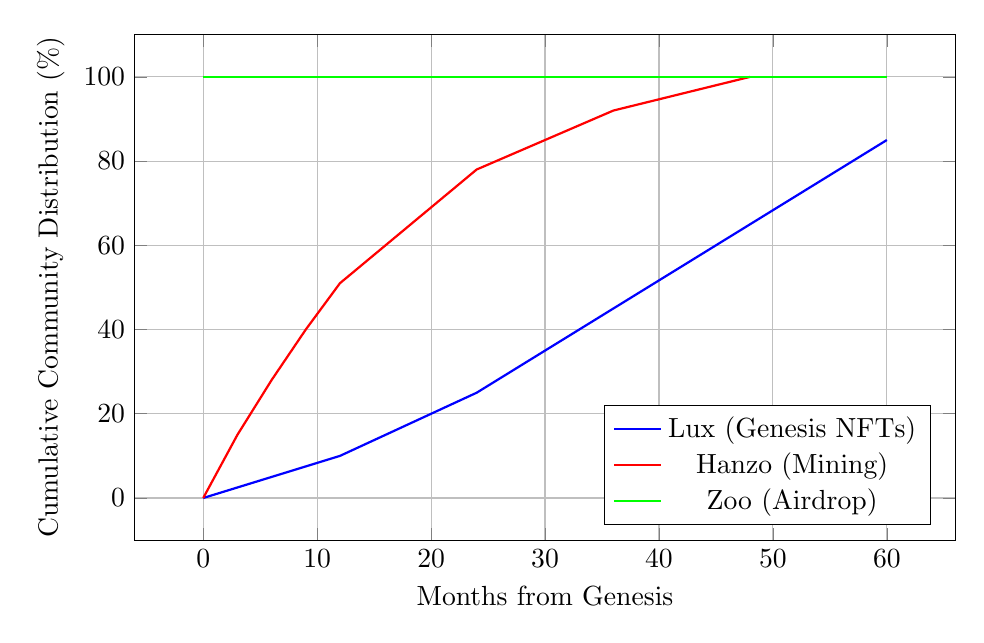
\begin{tikzpicture}
\begin{axis}[
    xlabel={Months from Genesis},
    ylabel={Cumulative Community Distribution (\%)},
    legend pos=south east,
    grid=major,
    width=12cm,
    height=8cm
]
\addplot[color=blue, thick] coordinates {
    (0,0) (12,10) (24,25) (36,45) (48,65) (60,85)
};
\addplot[color=red, thick] coordinates {
    (0,0) (3,15) (6,28) (9,40) (12,51) (24,78) (36,92) (48,100)
};
\addplot[color=green, thick] coordinates {
    (0,100) (12,100) (24,100) (36,100) (48,100) (60,100)
};
\legend{Lux (Genesis NFTs), Hanzo (Mining), Zoo (Airdrop)}
\end{axis}
\end{tikzpicture}
\caption{Cumulative community token distribution curves}
\label{fig:distribution_curves}
\end{figure}

Zoo's instant distribution creates immediate community ownership, avoiding the "who holds tokens controls early governance" problem that plagues gradual release models.

